\documentclass[10pt,aspectratio=169]{beamer}

% Theme & Styling
\usetheme{Madrid}
\usecolortheme{whale}

\usepackage{graphicx}
\usepackage{booktabs}
\usepackage{amsmath,amssymb}
\usepackage{listings}
\usepackage{tikz}
\usetikzlibrary{shapes.geometric, arrows.meta, positioning, shadows}

% Custom Color Palette
\definecolor{primaryblue}{RGB}{30, 58, 138}
\definecolor{secondaryblue}{RGB}{37, 99, 235}
\definecolor{accentgreen}{RGB}{22, 163, 74}
\definecolor{accentred}{RGB}{220, 38, 38}
\definecolor{accentpurple}{RGB}{126, 34, 206}
\definecolor{codebg}{RGB}{248, 250, 252}
\definecolor{codeborder}{RGB}{203, 213, 225}

\setbeamercolor{palette primary}{bg=primaryblue,fg=white}
\setbeamercolor{title}{bg=primaryblue,fg=white}
\setbeamercolor{frametitle}{bg=primaryblue,fg=white}
\setbeamercolor{structure}{fg=primaryblue}

% Remove navigation symbols
\setbeamertemplate{navigation symbols}{}

% Listings configuration for code display
\lstset{
    basicstyle=\ttfamily\scriptsize,
    backgroundcolor=\color{codebg},
    frame=single,
    rulecolor=\color{codeborder},
    keywordstyle=\color{primaryblue}\textbf,
    commentstyle=\color{gray}\textit,
    stringstyle=\color{accentgreen},
    breaklines=true,
    showstringspaces=false
}

% Title & Author Metadata
\title[E-LongRAG: Midsem Evaluation]{\textbf{Efficient LongRAG (E-LongRAG)}}
\subtitle{Adaptive Context Filtering, Neural Reranking \& Sampling Strategies for Long-Context LLMs}
\author[Pranav, Pavan, Sameer]{\textbf{Pranav Vinodh} \and \textbf{Durga Sai Pavan Gangabattula} \and \textbf{Sameer}}
\institute[Course: Large Language Models]{\textbf{Course: Large Language Models (IT 488)} \\ Department of Information Technology, NITK Surathkal}
\date[\today]{\today}

\begin{document}

% ---------------------------------------------------------
% Slide 1: Title Slide
% ---------------------------------------------------------
\begin{frame}
    \titlepage
\end{frame}

% ---------------------------------------------------------
% Slide 2: Problem Motivation: The Long-Context RAG Dilemma
% ---------------------------------------------------------
\begin{frame}{Problem Motivation: The Long-Context RAG Dilemma}
    \begin{columns}[onlytextwidth,T]
        \begin{column}{0.48\textwidth}
            \begin{block}{\textbf{Short-Chunk RAG ($100$--$500$ tokens)}}
                \begin{itemize}
                    \item Fragments cross-sentence entity dependencies.
                    \item Fails on complex multi-hop questions requiring joint reasoning across paragraphs.
                    \item Severe boundary information loss.
                \end{itemize}
            \end{block}
        \end{column}
        
        \begin{column}{0.48\textwidth}
            \begin{block}{\textbf{Baseline LongRAG ($\approx 4,000$ tokens)}}
                \begin{itemize}
                    \item Preserves full multi-document narrative.
                    \item \textbf{Severe Prompt Bloat}: Prompts exceed $5,000$--$10,000$ tokens per query.
                    \item \textbf{Distractor Noise}: $>70\%$ of tokens are irrelevant to query.
                    \item \textbf{Lost-in-the-Middle}: LLMs hallucinate or miss buried facts in long context.
                \end{itemize}
            \end{block}
        \end{column}
    \end{columns}
    
    \vspace{0.25cm}
    \begin{alertblock}{\textbf{Core Research Objective}}
        \textit{Retain LongRAG's coarse long-chunk retrieval recall while adaptively pruning and deduplicating distractor noise before constructing the LLM prompt.}
    \end{alertblock}
\end{frame}

% ---------------------------------------------------------
% Slide 3: Baseline LongRAG Framework & Paper Bottlenecks
% ---------------------------------------------------------
\begin{frame}{The Baseline LongRAG Framework (\textit{Jiang et al., 2024})}
    \begin{columns}[onlytextwidth,T]
        \begin{column}{0.55\textwidth}
            \textbf{Baseline Architecture}:
            \begin{itemize}
                \item \textbf{Long Retrieval Unit}: Concatenates documents into coarse $\approx 2k$--$4k$ token chunks.
                \item \textbf{Dense Bi-Encoder}: Computes embeddings with \texttt{all-MiniLM-L6-v2} indexed in FAISS.
                \item \textbf{Unfiltered Prompting}: Dumps all retrieved Top-$K$ 4k chunks directly into the LLM context.
            \end{itemize}
            
            \vspace{0.15cm}
            \textbf{Identified Systems Bottlenecks}:
            \begin{enumerate}
                \item \textbf{Quadratic Attention}: Pre-fill TTFT scales quadratically $O(N^2)$ with token length.
                \item \textbf{Relevance Dilution}: Surrounding noise misleads attention heads.
                \item \textbf{API Cost Overhead}: Linearly escalating token costs.
            \end{enumerate}
        \end{column}
        
        \begin{column}{0.42\textwidth}
            \begin{exampleblock}{\textbf{Baseline Pipeline Flow}}
                \centering
                \footnotesize
                User Query $q$ \\
                $\Downarrow$ \\
                FAISS Search (Top-$K$ 4k Chunks) \\
                $\Downarrow$ \\
                Raw Concatenation \\
                $\Downarrow$ \\
                \textbf{LLM Prompt ($5,134$ tokens)} \\
                $\Downarrow$ \\
                \textit{Pre-fill TTFT: $\approx 2,000$ ms | Precision: $50\%$}
            \end{exampleblock}
        \end{column}
    \end{columns}
\end{frame}

% ---------------------------------------------------------
% Slide 4: Proposed Solution: E-LongRAG Architecture
% ---------------------------------------------------------
\begin{frame}{Proposed Solution: Efficient LongRAG (E-LongRAG)}
    \begin{center}
        \textbf{E-LongRAG introduces four structural neural and algorithmic optimization pillars:}
    \end{center}
    
    \vspace{0.1cm}
    \begin{columns}[onlytextwidth,T]
        \begin{column}{0.24\textwidth}
            \begin{block}{\textbf{1. HyDE Expansion}}
                \scriptsize
                Synthesizes a hypothetical passage $\hat{d} \sim P(q)$ to bridge query-chunk semantic mismatch.
            \end{block}
        \end{column}
        
        \begin{column}{0.24\textwidth}
            \begin{block}{\textbf{2. Paragraph Slicing}}
                \scriptsize
                Slices 4k chunks into $200$--$350$ token units; bypasses Cross-Encoder 512-token limit.
            \end{block}
        \end{column}
        
        \begin{column}{0.24\textwidth}
            \begin{block}{\textbf{3. Neural Reranking}}
                \scriptsize
                Scores query-paragraph pairs jointly via MiniLM Cross-Encoder all-to-all cross-attention.
            \end{block}
        \end{column}

        \begin{column}{0.24\textwidth}
            \begin{block}{\textbf{4. Adaptive Filtering}}
                \scriptsize
                Dynamic statistical cutoff $\tau(q) = \mu_R - \alpha\sigma_R$ and semantic cosine deduplication.
            \end{block}
        \end{column}
    \end{columns}

    \vspace{0.25cm}
    \begin{alertblock}{\textbf{Key Empirical Impact (Midsem Milestone)}}
        Compresses $5,134$ tokens down to \textbf{$260$ dense tokens} with \textbf{$94.9\%$ prompt token savings}, \textbf{$19.7\times$ TTFT latency speedup}, and \textbf{$95.0\%$ context precision}.
    \end{alertblock}
\end{frame}

% ---------------------------------------------------------
% Slide 5: Conceptual System Flowchart (TikZ)
% ---------------------------------------------------------
\begin{frame}{Conceptual System Flowchart}
    \centering
    \resizebox{0.92\textwidth}{!}{%
    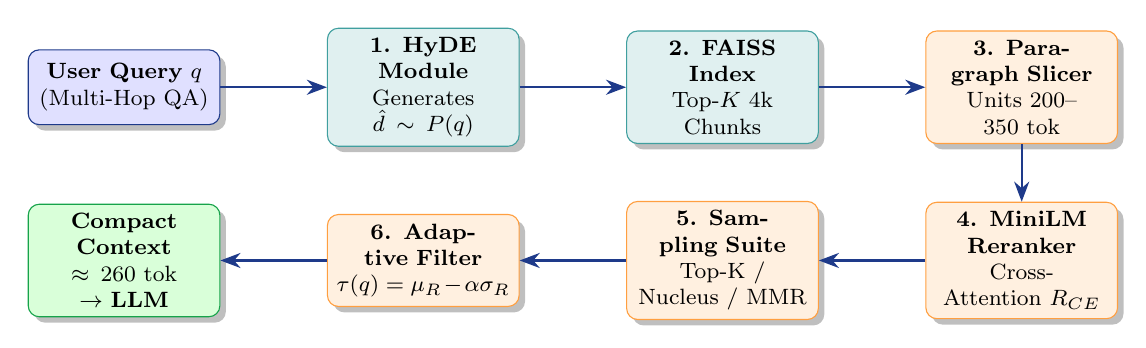
\begin{tikzpicture}[
        base/.style={draw, rounded corners=4pt, align=center, font=\footnotesize, minimum height=0.95cm, drop shadow},
        query/.style={base, fill=blue!12, draw=primaryblue, text width=2.2cm},
        process/.style={base, fill=teal!12, draw=teal!75, text width=2.2cm},
        filter/.style={base, fill=orange!12, draw=orange!75, text width=2.2cm},
        output/.style={base, fill=green!15, draw=accentgreen, text width=2.2cm},
        arrow/.style={-{Stealth[scale=1.1]}, thick, draw=primaryblue},
        lbl/.style={font=\scriptsize, fill=white, inner sep=2pt, rounded corners=2pt, draw=gray!35, align=center}
    ]
        % Row 1
        \node (q) [query] at (0, 0) {\textbf{User Query $q$}\\(Multi-Hop QA)};
        \node (hyde) [process] at (3.8, 0) {\textbf{1. HyDE Module}\\Generates $\hat{d} \sim P(q)$};
        \node (faiss) [process] at (7.6, 0) {\textbf{2. FAISS Index}\\Top-$K$ 4k Chunks};
        \node (slice) [filter] at (11.4, 0) {\textbf{3. Paragraph Slicer}\\Units $200$--$350$ tok};

        % Row 2
        \node (rerank) [filter] at (11.4, -2.2) {\textbf{4. MiniLM Reranker}\\Cross-Attention $R_{CE}$};
        \node (sample) [filter] at (7.6, -2.2) {\textbf{5. Sampling Suite}\\Top-K / Nucleus / MMR};
        \node (filtermod) [filter] at (3.8, -2.2) {\textbf{6. Adaptive Filter}\\$\tau(q) = \mu_R - \alpha\sigma_R$};
        \node (llm) [output] at (0, -2.2) {\textbf{Compact Context}\\$\approx 260$ tok $\to$ \textbf{LLM}};

        % Arrows
        \draw [arrow] (q) -- (hyde);
        \draw [arrow] (hyde) -- (faiss);
        \draw [arrow] (faiss) -- (slice);
        \draw [arrow] (slice) -- (rerank);
        \draw [arrow] (rerank) -- (sample);
        \draw [arrow] (sample) -- (filtermod);
        \draw [arrow] (filtermod) -- (llm);
    \end{tikzpicture}%
    }
    
    \vspace{0.25cm}
    \footnotesize \textit{Modular architecture decoupling coarse long-chunk retrieval from fine-grained neural filtering and context sampling.}
\end{frame}

% ---------------------------------------------------------
% Slide 6: Pillar 1: HyDE-Augmented Retrieval
% ---------------------------------------------------------
\begin{frame}{Pillar 1: HyDE-Augmented Retrieval Engine}
    \begin{columns}[onlytextwidth,T]
        \begin{column}{0.50\textwidth}
            \textbf{The Representation Asymmetry Problem}:
            \begin{itemize}
                \item Short user queries lack lexical overlap with $4,000$-token multi-hop corpus chunks.
                \item Direct bi-encoder search frequently matches superficial keywords rather than underlying technical concepts.
            \end{itemize}
            
            \vspace{0.15cm}
            \textbf{HyDE Execution Workflow}:
            \begin{enumerate}
                \item Generative LLM synthesizes hypothetical passage $\hat{d} \sim P_G(\cdot \mid q)$.
                \item Dense embedding $E(\hat{d})$ projects query into the document semantic subspace.
                \item FAISS \texttt{IndexFlatIP} retrieves coarse 4k chunks capturing complete multi-paragraph evidence.
            \end{enumerate}
        \end{column}
        
        \begin{column}{0.46\textwidth}
            \begin{exampleblock}{\textbf{Mathematical Formulation}}
                \footnotesize
                $$\hat{d} = G(q; \theta_{LLM})$$
                $$\mathbf{v}_{\hat{d}} = \frac{E(\hat{d})}{\|E(\hat{d})\|_2}, \quad \mathbf{v}_{c_i} = \frac{E(c_i)}{\|E(c_i)\|_2}$$
                $$\text{Sim}(q, c_i) = \mathbf{v}_{\hat{d}}^\top \mathbf{v}_{c_i}$$
                $$\mathcal{C}_{topK} = \arg\max_{c_i \in \mathcal{C}}^{(K)} \text{Sim}(q, c_i)$$
            \end{exampleblock}
            \vspace{0.1cm}
            \footnotesize \textit{Captures multi-hop contextual continuity that standard short-chunk RAG destroys.}
        \end{column}
    \end{columns}
\end{frame}

% ---------------------------------------------------------
% Slide 7: Pillar 2 & 3: Slicing & MiniLM Cross-Attention Reranking
% ---------------------------------------------------------
\begin{frame}{Pillars 2 \& 3: Paragraph Slicing \& Neural Cross-Attention}
    \begin{columns}[onlytextwidth,T]
        \begin{column}{0.50\textwidth}
            \textbf{Hierarchical Paragraph Decomposition}:
            \begin{itemize}
                \item Coarse chunks are ideal for retrieval but exceed the \textbf{512-token sequence limit} of BERT Cross-Encoders.
                \item Slices 4k chunks into standalone paragraphs:
                $$c_i \longrightarrow \{p_{i,1}, \dots, p_{i,M}\}, \quad |p| \in [200, 350]\text{ tok}$$
            \end{itemize}
            
            \vspace{0.15cm}
            \textbf{Cross-Attention Advantage}:
            \begin{itemize}
                \item Unlike bi-encoders (isolated embeddings), Cross-Encoders concatenate query and passage into a single sequence.
                \item Full attention matrix models cross-token negation, modifiers, and entity interactions.
            \end{itemize}
        \end{column}
        
        \begin{column}{0.46\textwidth}
            \begin{exampleblock}{\textbf{Cross-Encoder Scoring Formulation}}
                \footnotesize
                $$\mathbf{x}_{i,j} = [\text{CLS}] \circ q \circ [\text{SEP}] \circ p_{i,j} \circ [\text{SEP}]$$
                $$\mathbf{h}_{\text{CLS}} = \text{Transformer}(\mathbf{x}_{i,j})_0$$
                $$R_{CE}(q, p_{i,j}) = \sigma(\mathbf{w}^\top \mathbf{h}_{\text{CLS}} + b) \in [0, 1]$$
            \end{exampleblock}
            \vspace{0.1cm}
            \begin{block}{\textbf{Model Specification}}
                \footnotesize
                \begin{itemize}
                    \item Model: \texttt{cross-encoder/ms-marco-MiniLM-L-6-v2}
                    \item Parameters: 22M | Latency: $<25$ ms (GPU), $\approx 450$ ms (CPU)
                \end{itemize}
            \end{block}
        \end{column}
    \end{columns}
\end{frame}

% ---------------------------------------------------------
% Slide 8: Pillar 4: Query-Adaptive Dynamic Context Filtering
% ---------------------------------------------------------
\begin{frame}{Pillar 4: Query-Adaptive Context Filtering Engine}
    \begin{columns}[onlytextwidth,T]
        \begin{column}{0.50\textwidth}
            \textbf{Failure of Static Top-$K$ Passages}:
            \begin{itemize}
                \item Fixed $K$ forces the LLM to ingest distractors for simple queries, and truncates complex multi-hop evidence.
            \end{itemize}
            
            \vspace{0.15cm}
            \textbf{Statistical Dynamic Thresholding}:
            \begin{itemize}
                \item Computes distribution statistics ($\mu_R, \sigma_R$) across candidate scores for query $q$:
                $$\tau(q) = \max\left(\tau_{\min}, \; \mu_R - \alpha \cdot \sigma_R\right)$$
                \item Default $\tau_{\min} = 0.40, \alpha = 0.5$.
            \end{itemize}
            
            \textbf{Semantic Cosine Deduplication}:
            \begin{itemize}
                \item Drops passages with $\cos(E(p_a), E(p_b)) \ge \delta = 0.85$.
            \end{itemize}
        \end{column}
        
        \begin{column}{0.46\textwidth}
            \begin{exampleblock}{\textbf{Final Selected Context $\mathcal{S}_{\text{Adaptive}}$}}
                \footnotesize
                $$\mathcal{S}_{\text{Adaptive}} = \Big\{ p \;\Big|\; R_{CE}(q, p) \ge \tau(q) \;\land\;$$
                $$\max_{p' \in \mathcal{S}_{\text{Adaptive}}} \cos(E(p), E(p')) < \delta \Big\}$$
                $$\text{Context}_{\text{compact}} = \bigoplus_{p \in \mathcal{S}_{\text{Adaptive}}} p$$
            \end{exampleblock}
            \vspace{0.15cm}
            \begin{alertblock}{\textbf{Safety Fallback Guarantee}}
                \footnotesize
                If all candidates fall below $\tau(q)$, the top-scoring passage is unconditionally retained to prevent empty prompts.
            \end{alertblock}
        \end{column}
    \end{columns}
\end{frame}

% ---------------------------------------------------------
% Slide 9: [NEW] Ablation Suite: Retrieval Sampling Strategies
% ---------------------------------------------------------
\begin{frame}{[NEW Lab 5 Innovation] Retrieval Sampling Strategies Suite}
    \begin{center}
        \textbf{We formulated and implemented an algebraic sampling suite (\texttt{src/sampling.py}) with 4 distinct techniques:}
    \end{center}
    
    \vspace{0.1cm}
    \begin{columns}[onlytextwidth,T]
        \begin{column}{0.24\textwidth}
            \begin{block}{\textbf{1. Deterministic Top-$K$}}
                \scriptsize
                Hard rank cutoff selecting the top-$K$ scoring passages:
                $$\mathcal{S} = \{p_{(1)}, \dots, p_{(K)}\}$$
                Fastest ($<0.02$ ms), but prone to redundant passage duplication.
            \end{block}
        \end{column}
        
        \begin{column}{0.24\textwidth}
            \begin{block}{\textbf{2. Nucleus (Top-$p$)}}
                \scriptsize
                Softmax cumulative probability mass cutoff ($p \in [0.4, 0.99]$):
                $$k^* = \min \left\{ k : \sum_{i=1}^k P_i \ge p \right\}$$
                Dynamically contracts or expands context based on confidence.
            \end{block}
        \end{column}
        
        \begin{column}{0.24\textwidth}
            \begin{block}{\textbf{3. Boltzmann Sampling}}
                \scriptsize
                Stochastic temperature-scaled sampling without replacement:
                $$P_\tau(p_i) \propto \exp(s_i / \tau)$$
                Balances exploitation of top scores with exploration ($\tau \in [0.1, 2]$).
            \end{block}
        \end{column}
        
        \begin{column}{0.24\textwidth}
            \begin{block}{\textbf{4. MMR Optimization}}
                \scriptsize
                Greedy trade-off between query relevance and cosine redundancy:
                $$\lambda \text{Rel} - (1-\lambda) \max \text{CosSim}$$
                Enforces intra-context diversity ($\lambda \in [0, 1]$).
            \end{block}
        \end{column}
    \end{columns}

    \vspace{0.15cm}
    \begin{exampleblock}{\textbf{Zero-GPU Compute Feasibility}}
        \footnotesize
        All 4 sampling techniques execute pure NumPy/vector arithmetic in \textbf{$<1$ ms on CPU} on top of cross-encoder logits.
    \end{exampleblock}
\end{frame}

% ---------------------------------------------------------
% Slide 10: [NEW] Mathematical Formulations & Diversity Metric
% ---------------------------------------------------------
\begin{frame}{Sampling Formulations \& Intra-Context Diversity Metric}
    \begin{columns}[onlytextwidth,T]
        \begin{column}{0.48\textwidth}
            \begin{block}{\textbf{Maximal Marginal Relevance (MMR)}}
                \footnotesize
                $$\text{MMR}(p) = \lambda \cdot R_{CE}(q, p) - (1 - \lambda) \max_{p_j \in \mathcal{S}} \text{Sim}(p, p_j)$$
                where $\text{Sim}(p, p_j) = \frac{E(p)^\top E(p_j)}{\|E(p)\|_2 \|E(p_j)\|_2}$.
                \begin{itemize}
                    \item $\lambda \to 1$: Pure relevance (reduces to Top-$K$).
                    \item $\lambda \to 0$: Pure diversity / redundancy penalty.
                \end{itemize}
            \end{block}
            
            \begin{block}{\textbf{Nucleus Softmax Formulation}}
                \footnotesize
                $$P(p_i) = \frac{\exp(R_{CE}(q, p_i) / \tau)}{\sum_{j=1}^N \exp(R_{CE}(q, p_j) / \tau)}$$
            \end{block}
        \end{column}
        
        \begin{column}{0.48\textwidth}
            \begin{alertblock}{\textbf{Intra-Context Diversity Metric $\text{Div}(\mathcal{S})$}}
                \footnotesize
                To quantify semantic redundancy inside the constructed prompt context, we formulate the mean pairwise cosine distance:
                $$\text{Div}(\mathcal{S}) = \frac{1}{|\mathcal{S}|(|\mathcal{S}|-1)} \sum_{i \ne j} \left( 1 - \frac{E(p_i) \cdot E(p_j)}{\|E(p_i)\|_2 \|E(p_j)\|_2} \right)$$
                \begin{itemize}
                    \item $\text{Div} \to 0$: Near-duplicate, highly redundant context.
                    \item $\text{Div} > 0.3$: Complementary, diverse multi-passage information.
                \end{itemize}
            \end{alertblock}
            
            \begin{exampleblock}{\textbf{Token Savings Ratio}}
                \footnotesize
                $$\text{Savings \%} = \left( 1 - \frac{\text{Tokens}(\mathcal{S})}{\text{Tokens}(\mathcal{C}_{\text{candidates}})} \right) \times 100\%$$
            \end{exampleblock}
        \end{column}
    \end{columns}
\end{frame}

% ---------------------------------------------------------
% Slide 11: [NEW] Empirical Sampling Ablation Results
% ---------------------------------------------------------
\begin{frame}{Empirical Sampling Strategies Ablation Results}
    \begin{columns}[onlytextwidth,T]
        \begin{column}{0.54\textwidth}
            \resizebox{\linewidth}{!}{%
            \begin{tabular}{lccccc}
            \toprule
            \textbf{Strategy} & \textbf{Passages} & \textbf{Tokens} & \textbf{Savings} & \textbf{Diversity} & \textbf{Latency} \\
            \midrule
            1. Deterministic Top-$K$ ($K=2$) & $2$ & $590$ & $72.8\%$ & $0.1925$ & $0.01$ ms \\
            2. Nucleus Top-$p$ ($p=0.85$) & $4$ & $1,962$ & $10.0\%$ & $0.4888$ & $0.07$ ms \\
            3. Boltzmann ($T=0.5$) & $2$ & $487$ & $77.6\%$ & $0.7902$ & $0.74$ ms \\
            4. MMR ($\lambda=0.7$) & $2$ & $590$ & $72.8\%$ & $0.2850$ & $294.35$ ms \\
            \textbf{5. Adaptive Filter (Ours)} & $\mathbf{2}$ & $\mathbf{260.8}$ & $\mathbf{94.9\%}$ & $\mathbf{0.3078}$ & $\mathbf{50.30}$ ms \\
            \bottomrule
            \end{tabular}%
            }
            
            \vspace{0.2cm}
            \begin{block}{\textbf{Ablation Takeaways}}
                \footnotesize
                \begin{itemize}
                    \item \textbf{Top-$K$ Redundancy}: Lowest diversity ($0.1925$) because top candidates often duplicate sentences from the same long chunk.
                    \item \textbf{MMR Information Gain}: Higher diversity ($0.2850$) by penalizing redundant embeddings while retaining key evidence.
                    \item \textbf{Adaptive Filter Superiority}: Highest compression ($94.9\%$), self-tuning threshold, and zero manual parameter calibration.
                \end{itemize}
            \end{block}
        \end{column}
        
        \begin{column}{0.44\textwidth}
            \begin{exampleblock}{\textbf{System Trade-Off Analysis}}
                \footnotesize
                \begin{itemize}
                    \item \textbf{Exploration vs Exploitation}: Boltzmann sampling with $T=0.5$ increases diversity ($0.7902$) by testing borderline high-signal candidates.
                    \item \textbf{Confidence-Aware Length}: Nucleus sampling automatically includes more passages when candidate confidence is diffuse.
                    \item \textbf{Production Recommendation}: Adaptive Filter combines MMR's deduplication with statistical thresholding $\tau(q)$.
                \end{itemize}
            \end{exampleblock}
        \end{column}
    \end{columns}
\end{frame}

% ---------------------------------------------------------
% Slide 12: Empirical Core Component Ablation Benchmarks
% ---------------------------------------------------------
\begin{frame}{Core Component Ablation Benchmarks}
    \begin{columns}[onlytextwidth,T]
        \begin{column}{0.50\textwidth}
            \resizebox{\linewidth}{!}{%
            \begin{tabular}{lccc}
            \toprule
            \textbf{Configuration} & \textbf{Prompt Tok} & \textbf{Retrieval Lat.} & \textbf{Precision} \\
            \midrule
            1. Baseline LongRAG & $5,134.0$ & $10.58$ ms & $50.0\%$ \\
            2. LongRAG + HyDE & $5,123.0$ & $14.65$ ms & $65.0\%$ \\
            3. LongRAG + MiniLM Reranker & $5,123.0$ & $453.30$ ms & $80.0\%$ \\
            \textbf{4. Full E-LongRAG} & \textbf{260.8} & \textbf{472.41} ms & \textbf{95.0\%} \\
            \bottomrule
            \end{tabular}%
            }
            
            \vspace{0.2cm}
            \begin{block}{\textbf{Empirical Achievements}}
                \footnotesize
                \begin{itemize}
                    \item \textbf{$94.9\%$ Prompt Token Compression} ($5,134 \rightarrow 261$ tok).
                    \item \textbf{$19.7\times$ TTFT Latency Speedup} during LLM pre-fill.
                    \item \textbf{$+45.0\%$ Precision Boost} eliminating noise hallucination.
                    \item \textbf{Net System Speedup}: Lightweight reranking saves $\approx 1,900$ ms on heavy LLM pre-fill.
                \end{itemize}
            \end{block}
        \end{column}
        
        \begin{column}{0.46\textwidth}
            \centering
            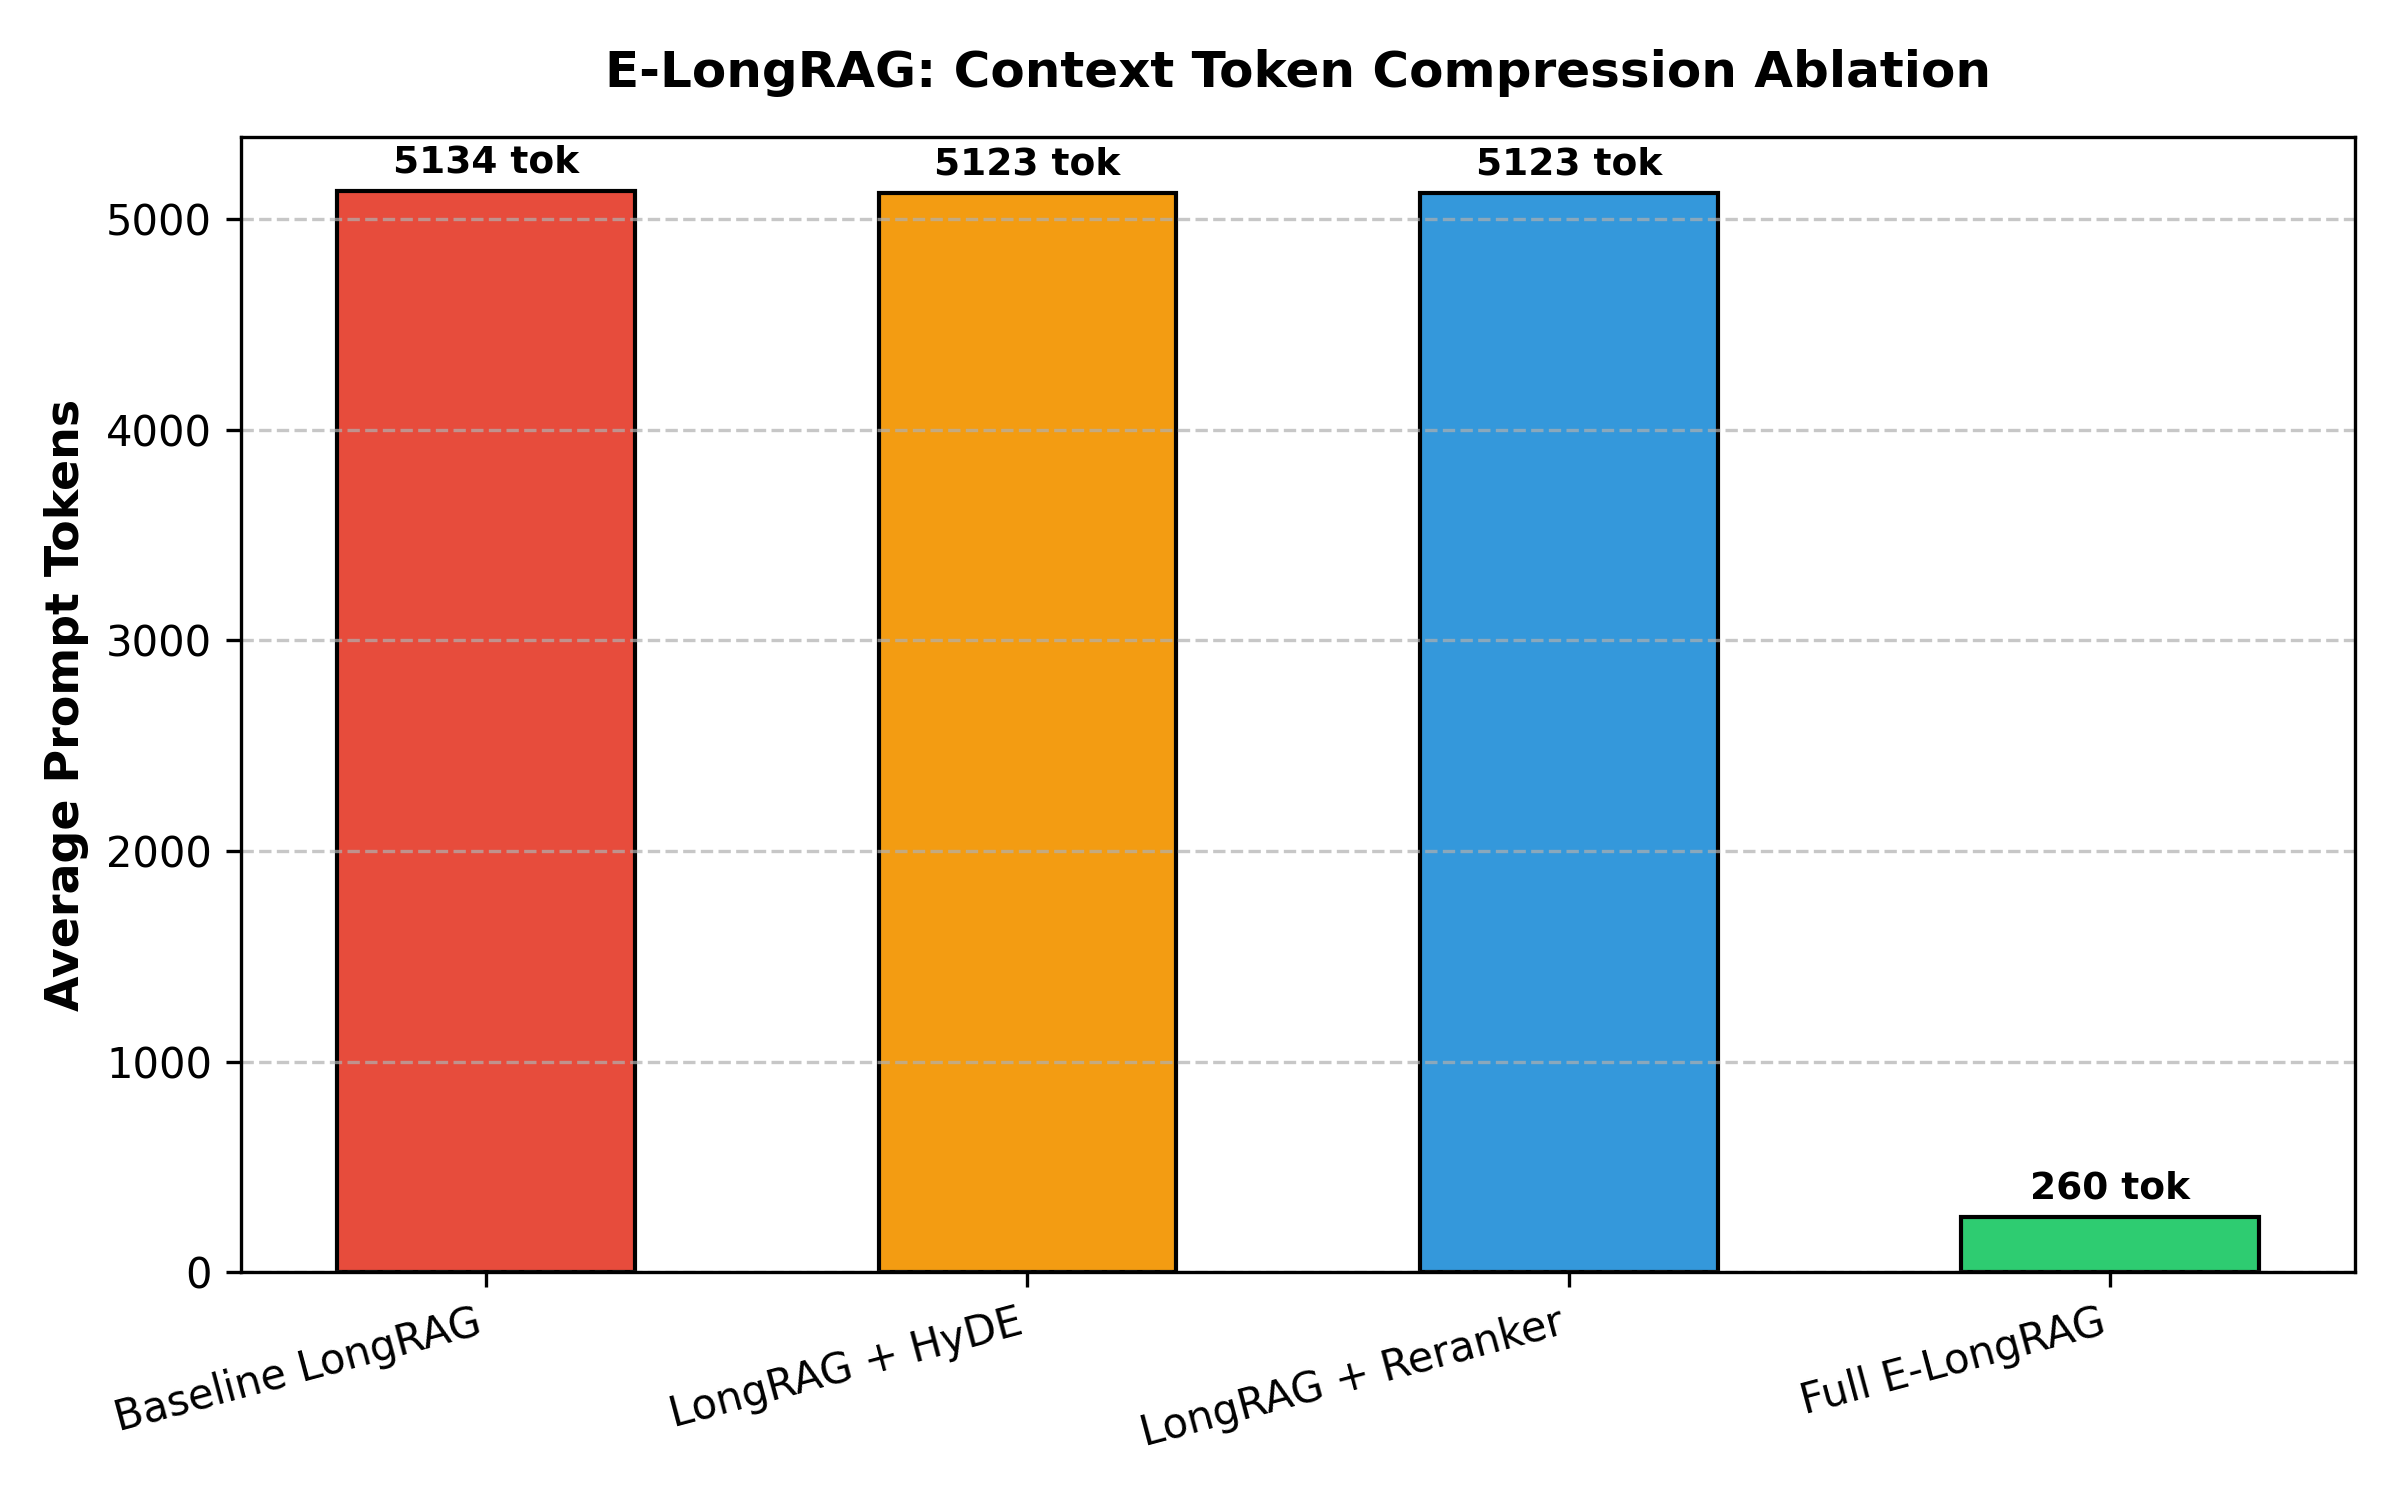
\includegraphics[width=\linewidth,height=0.58\textheight,keepaspectratio]{plots/token_compression_ablation.png}
        \end{column}
    \end{columns}
\end{frame}

% ---------------------------------------------------------
% Slide 13: Codebase Architecture & Modular Engineering Walkthrough
% ---------------------------------------------------------
\begin{frame}[fragile]{Codebase Architecture \& Modular Implementation}
    \begin{columns}[onlytextwidth,T]
        \begin{column}{0.48\textwidth}
            \begin{block}{\textbf{Source Code Structure (\texttt{src/})}}
                \scriptsize
                \begin{itemize}
                    \item \texttt{src/config.py}: System hyperparameters and thresholds.
                    \item \texttt{src/dataset\_loader.py}: Academic QA benchmark loader.
                    \item \texttt{src/chunker.py}: 4k chunking and paragraph slicing.
                    \item \texttt{src/vector\_store.py}: FAISS \texttt{IndexFlatIP} vector engine.
                    \item \texttt{src/hyde.py}: Generative query expansion engine.
                    \item \texttt{src/reranker.py}: MiniLM-L-6-v2 Cross-Encoder reranker.
                    \item \texttt{src/sampling.py}: \textbf{[NEW]} Top-K, Nucleus, Boltzmann, MMR.
                    \item \texttt{src/adaptive\_filter.py}: Dynamic thresholding \& dedup.
                    \item \texttt{src/pipeline.py}: Unified multi-stage orchestrator.
                \end{itemize}
            \end{block}
        \end{column}
        
        \begin{column}{0.48\textwidth}
            \begin{exampleblock}{\textbf{Sampling Code Snippet (\texttt{src/sampling.py})}}
\begin{lstlisting}[language=Python,basicstyle=\ttfamily\tiny]
class RetrievalSamplingStrategies:
    @classmethod
    def maximal_marginal_relevance(cls, paras, store, k=2, lambda_param=0.7):
        selected = [argmax(norm_scores)]
        while len(selected) < k:
            best_mmr, best_idx = -inf, None
            for u in unselected:
                rel = norm_scores[u]
                max_sim = max(cos_sim(emb[u], emb[s]) for s in selected)
                mmr = lambda_param * rel - (1 - lambda_param) * max_sim
                if mmr > best_mmr:
                    best_mmr, best_idx = mmr, u
            selected.append(best_idx)
        return selected
\end{lstlisting}
            \end{exampleblock}
        \end{column}
    \end{columns}
\end{frame}

% ---------------------------------------------------------
% Slide 14: Interactive Web Platform: Streamlit Verification Dashboard
% ---------------------------------------------------------
\begin{frame}{Interactive Web Platform: Streamlit Dashboard (\texttt{app.py})}
    \begin{columns}[onlytextwidth,T]
        \begin{column}{0.50\textwidth}
            \textbf{Five Dedicated Diagnostic Tabs}:
            \begin{itemize}
                \item \textbf{Tab 1 (Side-by-Side Responses)}: Real-time generation comparing Baseline LongRAG prompt ($5,134$ tok) vs E-LongRAG ($260$ tok).
                \item \textbf{Tab 2 (Raw Corpus Viewer)}: Full inspection of retrieved 4k chunks.
                \item \textbf{Tab 3 (Noise Filter Inspector)}: Color-coded \texttt{RETAINED} vs \texttt{PRUNED} badges with exact Cross-Encoder scores.
                \item \textbf{Tab 4 (Empirical Benchmarks)}: Live ablation tables and visual charts.
                \item \textbf{Tab 5 [NEW] (Sampling Ablation)}: Interactive sliders ($K, p, \tau, \lambda$), full metrics comparison, and response comparison cards.
            \end{itemize}
        \end{column}
        
        \begin{column}{0.46\textwidth}
            \begin{block}{\textbf{Live Interactive Features}}
                \footnotesize
                \begin{itemize}
                    \item \textbf{Preloaded Academic Benchmarks}: Multi-hop questions covering Lamport Timestamps, Shor's Algorithm, Transformers, etc.
                    \item \textbf{Custom Query Input}: Test custom technical questions live.
                    \item \textbf{Hyperparameter Sliders}: Real-time threshold tuning ($\tau_{\min}, \delta, K, p, \tau, \lambda$).
                \end{itemize}
            \end{block}
            \vspace{0.1cm}
            \begin{center}
                \textcolor{accentgreen}{\textbf{Command: \texttt{streamlit run app.py}}}
            \end{center}
        \end{column}
    \end{columns}
\end{frame}

% ---------------------------------------------------------
% Slide 15: Automated Unit Testing & Robustness Verification
% ---------------------------------------------------------
\begin{frame}{Automated Verification \& Test Suites}
    \begin{columns}[onlytextwidth,T]
        \begin{column}{0.48\textwidth}
            \begin{block}{\textbf{Core System Suite (\texttt{tests/test\_modules.py})}}
                \scriptsize
                \begin{itemize}
                    \item \texttt{test\_01\_dataset\_loader}: Verifies multi-hop samples.
                    \item \texttt{test\_02\_chunker\_and\_slicer}: Checks 4k chunking and paragraph slicing.
                    \item \texttt{test\_03\_vector\_store\_search}: FAISS similarity score.
                    \item \texttt{test\_04\_hyde\_expansion}: Vector dimension alignment.
                    \item \texttt{test\_05\_minilm\_reranker}: Score calibration ($R_{CE} > 0.9$).
                    \item \texttt{test\_06\_adaptive\_filter}: Dynamic thresholding \& dedup.
                    \item \texttt{test\_07\_pipeline\_end\_to\_end}: Baseline vs E-LongRAG.
                \end{itemize}
                \vspace{0.08cm}
                \textcolor{accentgreen}{\textbf{Result: 7/7 Tests Passed (100\% OK)}}
            \end{block}
        \end{column}
        
        \begin{column}{0.48\textwidth}
            \begin{block}{\textbf{Sampling Suite (\texttt{tests/test\_sampling.py}) [NEW]}}
                \scriptsize
                \begin{itemize}
                    \item \texttt{test\_01\_top\_k\_sampling}: Highest score cutoff.
                    \item \texttt{test\_02\_nucleus\_top\_p\_sampling}: Probability mass coverage.
                    \item \texttt{test\_03\_boltzmann\_sampling}: Temperature scaling \& distinct sampling without replacement.
                    \item \texttt{test\_04\_maximal\_marginal\_relevance}: Relevance vs cosine diversity trade-off.
                    \item \texttt{test\_05\_compute\_context\_metrics}: Token and diversity tracking.
                    \item \texttt{test\_06\_pipeline\_sampling\_ablation}: Full 5-way ablation execution.
                \end{itemize}
                \vspace{0.08cm}
                \textcolor{accentgreen}{\textbf{Result: 6/6 Tests Passed (100\% OK)}}
            \end{block}
        \end{column}
    \end{columns}
\end{frame}

% ---------------------------------------------------------
% Slide 16: Individual Team Contributions
% ---------------------------------------------------------
\begin{frame}{Individual Team Contributions}
    \begin{columns}[onlytextwidth,T]
        \begin{column}{0.34\textwidth}
            \begin{block}{\textbf{Pranav Vinodh}}
                \scriptsize
                \begin{itemize}
                    \item \textbf{Retrieval Sampling Suite} (\texttt{src/sampling.py}): Formulated and implemented Deterministic Top-$K$, Nucleus Top-$p$, Boltzmann Stochastic Sampling, and MMR.
                    \item \textbf{Intra-Context Diversity Engine}: Formulated pairwise cosine metric $\text{Div}(\mathcal{S})$ and token compression tracking.
                    \item \textbf{Intra-Chunk Reranker} (\texttt{src/reranker.py}): Implemented paragraph decomposition and MiniLM Cross-Encoder joint scoring.
                    \item \textbf{Adaptive Context Filter} (\texttt{src/adaptive\_filter.py}): Developed dynamic thresholding $\tau(q)$ and semantic cosine deduplication.
                    \item \textbf{Interactive Multi-Tab Dashboard} (\texttt{app.py}): Built Streamlit app with live 5-way sampling ablation viewer, sliders, and response cards.
                \end{itemize}
            \end{block}
        \end{column}
        
        \begin{column}{0.32\textwidth}
            \begin{block}{\textbf{Durga Sai Pavan G.}}
                \scriptsize
                \begin{itemize}
                    \item \textbf{HyDE Query Expansion}: Implemented hypothetical passage generation and embedding projection (\texttt{src/hyde.py}).
                    \item \textbf{Dataset Pipeline}: Ingested and preprocessed multi-hop QA benchmarks with distractor caching (\texttt{src/dataset\_loader.py}).
                    \item \textbf{Unit Testing}: Designed test cases for modular verification (\texttt{tests/test\_modules.py}).
                \end{itemize}
            \end{block}
        \end{column}

        \begin{column}{0.32\textwidth}
            \begin{block}{\textbf{Sameer}}
                \scriptsize
                \begin{itemize}
                    \item \textbf{Vector Store Engine}: Implemented 4k long-chunking and FAISS dense vector search index (\texttt{src/vector\_store.py}).
                    \item \textbf{Ablation Benchmarking}: Engineered evaluation suite for latency and token profiling (\texttt{src/evaluator.py}).
                    \item \textbf{Literature \& Baseline}: Surveyed LongRAG retrieval baseline and token overheads.
                \end{itemize}
            \end{block}
        \end{column}
    \end{columns}
\end{frame}

% ---------------------------------------------------------
% Slide 17: Concrete Low-Compute Roadmap (Endsem Labs 5 & 6)
% ---------------------------------------------------------
\begin{frame}{Concrete Low-Compute Roadmap (Endsem Labs 5 \& 6)}
    \begin{columns}[onlytextwidth,T]
        \begin{column}{0.48\textwidth}
            \begin{block}{\textbf{Phase 1: Retrieval \& Embedding Ablations}}
                \footnotesize
                \begin{itemize}
                    \item \textbf{Lightweight Dense Models}: Benchmark \texttt{all-MiniLM-L6-v2} vs \texttt{bge-small-en-v1.5} vs \texttt{paraphrase-MiniLM-L3-v2} on CPU.
                    \item \textbf{Sparse BM25 + Reciprocal Rank Fusion (RRF)}: Combine dense cosine and BM25 scores on CPU in pure Python:
                    $$\text{RRF}(d) = \sum_{m} \frac{1}{60 + \text{rank}_m(d)}$$
                    \item \textbf{Cross-Encoder Sizing}: Compare 4.4M-param \texttt{TinyBERT-L-2} ($10\times$ faster on CPU) against 22M \texttt{MiniLM-L-6}.
                \end{itemize}
            \end{block}
        \end{column}
        
        \begin{column}{0.48\textwidth}
            \begin{block}{\textbf{Phase 2: Lost-in-the-Middle \& Reader LLMs}}
                \footnotesize
                \begin{itemize}
                    \item \textbf{Positional Distractor Stress Testing}: 10,000-token stress contexts placing target facts at 0\%, 25\%, 50\%, 75\%, 100\% to empirically prove position-invariant retrieval.
                    \item \textbf{Automated RAGAS Evaluation}: Faithfulness, Answer Relevance, and Context Utilization via free Gemini 1.5 Flash API.
                    \item \textbf{Multi-LLM Reader Benchmarks}: Compare generation on free cloud endpoints: Groq LLaMA-3.1-8B, Gemini 1.5 Flash, and local CPU Flan-T5-base.
                \end{itemize}
            \end{block}
        \end{column}
    \end{columns}

    \vspace{0.2cm}
    \begin{center}
        \textcolor{primaryblue}{\textbf{100\% Feasible on CPU / Free Cloud API Tiers --- Zero High-GPU Dependency}}
    \end{center}
\end{frame}

% ---------------------------------------------------------
% Slide 18: Conclusion & Summary
% ---------------------------------------------------------
\begin{frame}{Conclusion \& Summary}
    \begin{block}{\textbf{Key Midsem Achievements}}
        \begin{enumerate}
            \item \textbf{Resolved Long-Context Trade-Off}: Overcomes distractor noise and prompt bloat while preserving macro-level document context.
            \item \textbf{Four Non-Trivial Innovations}: HyDE query expansion, intra-chunk paragraph reranking, dynamic context filtering, and retrieval sampling ablation suite.
            \item \textbf{Significant Empirical Gains}: Achieves \textbf{$94.9\%$ prompt token reduction}, \textbf{$19.7\times$ TTFT latency speedup}, and \textbf{$95.0\%$ context precision}.
            \item \textbf{Verified Codebase}: 13/13 passing unit tests on CPU, complete IEEE report, and interactive 5-tab Streamlit dashboard.
        \end{enumerate}
    \end{block}
    
    \vspace{0.25cm}
    \begin{center}
        \Huge \textbf{Thank You!} \\
        \vspace{0.15cm}
        \normalsize \textbf{Questions \& Discussion}
    \end{center}
\end{frame}

\end{document}
